% Chapter 1
\chapter{Introducción general} % Main chapter title

Este capitulo explica los motivos detrás de la decisión de realizar este Trabajo Final. 
Enumera los alcances y requerimientos del proyecto. Y Realiza una comparación entre el dispositivo desarrollado y productos de características similares que están disponibles en el mercado.

\label{Chapter1} % For referencing the chapter elsewhere, use \ref{Chapter1} 
\label{IntroGeneral}

%----------------------------------------------------------------------------------------

% Define some commands to keep the formatting separated from the content 
\newcommand{\keyword}[1]{\textbf{#1}}
\newcommand{\tabhead}[1]{\textbf{#1}}
\newcommand{\code}[1]{\texttt{#1}}
\newcommand{\file}[1]{\texttt{\bfseries#1}}
\newcommand{\option}[1]{\texttt{\itshape#1}}
\newcommand{\grados}{$^{\circ}$}

%----------------------------------------------------------------------------------------

%\section{Introducción}

%----------------------------------------------------------------------------------------
\section{Motivación}

Desde el año 1991 en adelante, todos los fabricantes de vehículos de combustión interna están obligados a incluir en sus vehículos un sistema electrónico de diagnóstico. Este sistema, conocido por sus siglas en inglés como OBD (On-Board Diagnostics), realiza las tareas de muestrear sensores que están conectados físicamente sobre el motor y alertar al conductor, a través de un indicador en el tablero, cuando el motor no está funcionando dentro de los parámetros de operación. También mantiene un registro interno de los fallos ocurridos durante la vida del mismo, para luego ser descargado por el mecánico encargado de realizar tareas de reparación o puesta a punto, y así facilitar su trabajo.
Actualmente existen grupos de entusiastas y coleccionistas que poseen vehículos fabricados antes de que el sistema OBD se haga obligatorio. Y por esa razón, no tienen la posibilidad de hacer un monitoreo del funcionamiento del motor de su vehículo. Tampoco es posible mantener un registro de si hubo eventos de fallas o momentos de operación fuera de rango, información útil para su mantenimiento preventivo.
Por esto es que se tomó la decisión de desarrollar para este Trabajo Final, un dispositivo que cumpla las mismas funciones que un OBD, pero para vehículos antiguos que no tienen instalado dicho sistema de fábrica.

\section{Alcance y objetivos}

El objetivo de este trabajo final fue de desarrollar un prototipo que realizara las funciones de muestrear, guardar y mostrar en tiempo real, los datos adquiridos por los sensores del motor.

\subsection{Alcances}

Los alcances de el Trabajo Final son:
\begin{itemize}
\item La elección de componentes electrónicos
\item El diseño del circuito para amplificar las señales de los sensores.
\item El diseño del circuito impreso.
\item El desarrollo del firmware de la parte adquisidora.
\item El desarrollo del software de la interfáz gráfica de usuario.
\item La confección de un primer prototipo.
\item Los ensayos de verificación y validación con el prototipo.
\end{itemize}

Quedan excluídas las siguientes tareas para una siguiente etapa del proyecto:
\begin{itemize}
\item La elección o desarrollo de un gabinete para la parte adquisidora.
\item El desarrollo de los componentes de montaje del sistema adquisidor.
\item El montaje del dispositivo para la interfáz gráfica.
\item Desarrollo del embalaje y documentación acompañante (e.g.: manual de usuario, prospecto)
\end{itemize}

La selección de los sensores a utilizar no formó parte de el Trabajo Final porque los sensores fueron seleccionados previo al comienzo del desarrollo.

\subsection{Requerimientos}
El Trabajo Final fue planificado según los siguientes requisitos que se divieron en cuatro grupos: Requerimientos generales del proyecto; requerimientos de la interfáz gráfica; requerimientos de la parte adquisidora de datos y requerimientos de la comunicación entre las partes.

Los requerimientos generales del proyecto son:
\begin{itemize}
\item REQ-GEN-001: Todo el código fuente del proyecto será almacenado bajo un sistema de control de versiones GIT.
\item REQ-GEN-002: La documentación del código fuente del sfotware embebidos será llevada a cabo en los comentarios, siguiendo el formato de Doxygen.
\item REQ-GEN-003: La documentación del software para la interfaz gráfica también será llevada a cabo en los comentarios. El formato será elegido por el responsable del proyecto.
\end{itemize}

Requerimientos de la interfáz gráfica:
\begin{itemize}
\item REQ-GUI-001: La interfaz gráfica deberá poder mostrar figuras con la información de todos los sensores a la vez.
\item REQ-GUI-002: El usuario tiene que poder elegir qué sensores ver al mismo tiempo y cuáles no desea ver.
\item REQ-GUI-003: El usuario tiene que poder definir alarmas por valor máximo, para cada una de las variables.
\item REQ-GUI-004: Las alarmas serán sonores y visuales. El estilo de las alarmas será definido por el cliente durante el proceso de desarrollo de la interfáz gráfica.
\end{itemize}

Requerimientos de la parte adquisidora:
\begin{itemize}
\item REQ-ADQ-001: El sistema tiene que adquirir la temperatura de los gases de admisión y escape, con un rango de temperatura entre 0\degree C y 400 \degree C y con una resolución menor igual a 0,5\degree C. Con una tasa de muestreo mayor o igual a 1hz.
\item REQ-ADQ-002: El sistema tiene que adquirir la temperatura del aceite del motor, con un rango de temperatura entre 0\degree C y 400\degree C y una resolución menor igual a 0,5\degree C. Con una tasa de muestreo mayor igual a 1hz.
\item REQ-ADQ-003: El sistema tiene que adquirir la velocidad de giro del motor, en un rango entre 0 y 20.000 revoluciones por minuto, con una resolución menor igual a 500 r.p.m. Con una tasa de muestreo mayor igual a 5hz.
\item REQ-ADQ-004: El sistema tiene que adquirir la proporción de oxígeno en los gases de escape llamada lambda, con un rango de 0 a 2 y una resolución menor igual a 0,1 lambda.
\item REQ-ADQ-005: El sistema tiene que adquirir la presión de aceite del motor, con un rango de 0 a 100 psi y con una resolución menor igual a 1 psi.
\item REQ-ADQ-006: El sistema debe comenzar a transmitir a la interfaz gráfica la información obtenida en un tiempo no mayor a 1 segundo transcurrido el proceso de adquisición.
\end{itemize}

Requerimientos de la comunicación entre las partes del sistema:
\begin{itemize}
\item REQ-COMM-001: Se permitirá que se pierda hasta 1 paquete de cada 100 paquetes transmitidos.
\end{itemize}


\section{Estado del arte}

Actualmente en el mercado existen productos de características y funcionalidades similares. Para poder hacer una comparación se eligieron los productos de entrada de dos marcas distintas. Uno es el Fueltech FT-300, que puede verse en la figura \ref{fig:comparativa} \subref{fig:fueltech},  y el otro es el HT-193000 de Halltech, visto en la figura \ref{fig:comparativa}\subref{fig:halltech}. La tabla \ref{tab:comparativa} hace una comparativa entre estos productos y el dispositivo desarrollado para el Trabajo Final, enlistando sus funcionalidades y características. Cabe destacar que al momento de escribir esta memoria, no existen un producto de estas características que esté diseñado o fabricado en Argentina.

\begin{figure}[htpb]
\centering
\begin{subfigure}{.4\textwidth}
\centering
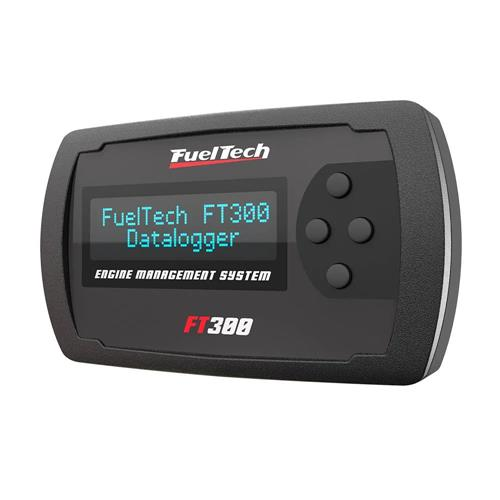
\includegraphics[width=\textwidth]{./Figures/fueltech-ft300.jpg}
\caption{Fueltech FT-300}
\label{fig:fueltech}
\end{subfigure}
\hfill
\begin{subfigure}{.5\textwidth}
\centering
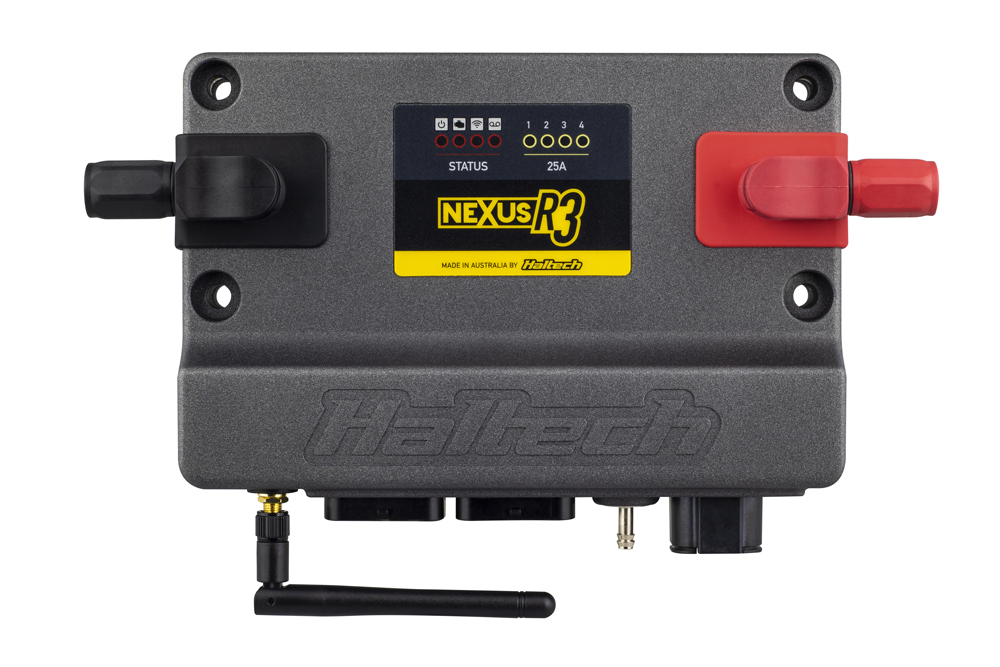
\includegraphics[width=\textwidth]{./Figures/HT-193000_00.JPG}
\caption{Halltech HT-193000}
\label{fig:halltech}
\end{subfigure}
\hfill
\caption{Fotografias de ambas ECUs, a la izquierda (A) se ve la ECU FT-300 de Fueltech, y a la derecha (B) se ve la ECU HT-193000 de Halltech.}
\label{fig:comparativa}
\end{figure}
\hfil
\begin{table}[h]
	\centering
	\caption[Tabla comparativa entre dispositivos]{Tabla comparativa entre dispositivos}
	\centering
	\begin{tabular}{l c c c}    
		\toprule
		\textbf{Característica }     & \textbf{HT-193000} & \textbf{FT-300} & \textbf{Trabajo Final}\\
		\midrule
		Entradas temperatura	&  0 &   2 &  3\\
		Presión de aceite		& Si &  Si & Si\\
		Presión de combustible	& Si &  Si & No\\
		Presión de admisión		& Si &  Si & No\\
		Sonda Lambda			& Si &  Si & Si\\
		R.P.M.					& Si &  Si & Si\\
		Entradas analógicas		& 11 &  0  &  0\\
		Control de inyección	& Si &  Si & No\\
		Interfáz gráfica		& No &  Matriz de puntos & Pantalla LCD \\
		\bottomrule
	\end{tabular}
	\label{tab:comparativa}
\end{table}

Como se puede ver de la tabla \ref{tab:comparativa} el prototipo desarrollado no posee entradas para presión de combustible, presión de admisión y tampoco posee control de inyección, como los otros dos productos. Se decidió no implementar estas características para abaratar costos y no alargar el tiempo de desarrollo. La ventaja que tiene el prototipo es que tiene una pantalla LCD para mostrar las gráficas de las evoluciones de las variables en el tiempo.
